\documentclass[11pt]{article}
\addtolength{\oddsidemargin}{-1.cm}
\addtolength{\textwidth}{2cm}
\addtolength{\topmargin}{-2cm}
\addtolength{\textheight}{3.5cm}

\usepackage[pdftex]{graphicx}
\usepackage{hyperref}
\usepackage{float}
\usepackage{cite}
\hypersetup{
	colorlinks=true,
	linkcolor=black,
	filecolor=magenta,
	urlcolor=cyan,
}

% define the title
\author{Team Kahki}
\title{Requirements Specification}

\begin{document}
	\setlength{\parskip}{6pt}
	
	% generates the title
	\begin{titlepage}
	
	\begin{center}
		% Upper part of the page       
		
\includegraphics[width=0.7\linewidth]{Images/uniLogo.jpg}\\[1cm]    
		\textsc{\LARGE Khaki Round1}\\[0.3cm]
		
\includegraphics[width=0.5\linewidth]{Images/TeamLogoSmall.jpg}\\[0.5cm]
		% Title
		\rule{\linewidth}{0.5mm} \\[1cm]
		{ \huge \bfseries Requirements Specification}\\[0.5cm]
		\rule{\linewidth}{0.5mm} \\[1cm] 			
		
		\begin{minipage}{0.4\textwidth}
			\begin{flushleft} \large
				Kulani {Bamuza}
			\end{flushleft}
		\end{minipage}
		\begin{minipage}{0.4\textwidth}
			\begin{flushright} \large
				\emph{} \\
				15008402 
			\end{flushright}
		\end{minipage}
		
		
		\begin{minipage}{0.4\textwidth}
			\begin{flushleft} \large
				\emph{} \\
				Frederick {Ehlers}
			\end{flushleft}
		\end{minipage}
		\begin{minipage}{0.4\textwidth}
			\begin{flushright} \large
				\emph{} \\
				11061112
			\end{flushright}
		\end{minipage}
		
		
		\begin{minipage}{0.4\textwidth}
			\begin{flushleft} \large
				\emph{} \\
				Dimpho {Mahoko}
			\end{flushleft}
		\end{minipage}
		\begin{minipage}{0.4\textwidth}
			\begin{flushright} \large
				\emph{} \\
				15175091
			\end{flushright}
		\end{minipage}

		\begin{minipage}{0.4\textwidth}
			\begin{flushleft} \large
				\emph{} \\
				Katlego {Mogokonyane}
			\end{flushleft}
		\end{minipage}
		\begin{minipage}{0.4\textwidth}
			\begin{flushright} \large
				\emph{} \\
				12134229
			\end{flushright}
		\end{minipage}

		\begin{minipage}{0.4\textwidth}
			\begin{flushleft} \large
				\emph{} \\
				Maria {Qumayo}
			\end{flushleft}
		\end{minipage}
		\begin{minipage}{0.4\textwidth}
			\begin{flushright} \large
				\emph{} \\
				29461775
			\end{flushright}
		\end{minipage}

		\begin{minipage}{0.4\textwidth}
			\begin{flushleft} \large
				\emph{} \\
				Craig van Heerden
			\end{flushleft}
		\end{minipage}
		\begin{minipage}{0.4\textwidth}
			\begin{flushright} \large
				\emph{} \\
				15029779
			\end{flushright}
		\end{minipage}

		\begin{minipage}{0.4\textwidth}
			\begin{flushleft} \large
				\emph{} \\
				Linda {Zwane}
			\end{flushleft}
		\end{minipage}
		\begin{minipage}{0.4\textwidth}
			\begin{flushright} \large
				\emph{} \\
				14199468
			\end{flushright}
		\end{minipage}
		
		\textsc{\Large Stakeholders}\\[1cm]	
		
		\begin{minipage}{0.4\textwidth}
			\begin{flushleft} \large
				\emph{} \\
				Computer Science Department of University of Pretoria
			\end{flushleft}
		\end{minipage}
		\begin{minipage}{0.4\textwidth}
			\begin{flushright} \large
				\emph{} \\
				Vreda Pieterse
			\end{flushright}
		\end{minipage}
		
	\end{center}
\end{titlepage}
	
	\tableofcontents
	
	\newpage
	\section{Introduction}
	The introduction of the Software Requirements Specification provides an overview of the entire specification with purpose, scope, definitions, acronyms, abbreviations, references and overview of the SRS. The aim of this document is to define the problem in detail and provide the detailed requirements for NavUP.
	
	\subsection{Purpose}
	The purpose of this SRS document is to provide a detailed description of NavUP by collecting and analyzing the ideas that define the system. This document describes NavUP’s user interface, External Interface, functional, and performance requirements. The document also describes the users of NavUp and its functions. The document helps developers of the NavUp system in software delivery lifecycle processes. 

	\subsection{Scope}
	The product as mentioned before is called NavUP, nav being an abbreviation for navigation and UP is an acronym for University of Pretoria.
	The product should be available on all major mobile operating systems to ensure most users can use the product.
	The basic functionality of the product should be similar to the basic functionalities of navigation systems like Google Maps and Waze. It should be able to provide the user with their current location, it should be able to to search for locations and venues, it should be able to provide the user with navigation to a location or venue, and it should be able to save locations or venues. 
	
	The system must be able to provide the user their location outdoors as well as indoors. GPS will therefore not suffice because the GPS receiver will not be able to receive a signal indoors. The system will therefore only use Wi-Fi and crowdsourcing to determine the user's location.
	
	The system should also have different levels of users, users with higher levels should be able to add new locations into the system. These locations can include points of interest, events and activities.
	
	The system should be able to give the user information about how busy certain areas of the campus are. This can shown to the user visually through a heat map.
	
	The system should also give users notifications based on their current location like points of interest. The system can learn what type of locations the user likes based on their previous locations and suggest them new locations to visit. The system should also record the user's movement data and reward them in a game like fashion. 
	
	    The intended users are all students, staff and guests of the University of Pretoria. They should be able to navigate around campus, shown heat maps and get notifications based on their locations.
	
	\subsection{Definitions, Acronyms, and Abbreviations}
	\begin{table}[]
		\centering
		\resizebox{\textwidth}{!}{%
			\begin{tabular}{|l|l|}
				\hline
				GPS           & Global Positioning System. Used to determine a location on earth using satelite.                                     \\ \hline
				Accelerometer & An instrument for measuring the acceleration of a moving or vibrating body.                                          \\ \hline
				Heat map      & Visual dashboard that shows the concentration of subject of interest (pedestrian traffic) computed statistically.    \\ \hline
				Wi-Fi         & Wireless Fidelity. A form of wireless network communication.                                                         \\ \hline
				GUI           & Graphical User Interface where a user can interact with the system by making inputs, searching and getting outputs. \\ \hline
			\end{tabular}%
		}
	\end{table}

	\subsection{References}
	\begin{itemize}
		\item Higher Specification
	\end{itemize}

	\subsection{Overview}
	The remaining sections of this document describes the context of the product, summary of the product’s functions, describes the characteristics of the users, outlines the restrictions of the solution space, lists the factors that affect the requirements, and it describes the software requirements including external interface requirements, functional requirements,  and performance requirements. Section 2 provides an overview of the product. Section 3 provides a detailed description for each of the system interfaces, provides a detailed description of the products functionality, describes all the performance related capabilities of the product and outlines all the restrictions. 

	\section{ Specific Requirements }
	
	\subsection{Functional Requirements:}
	
	\subsubsection{Functional Requirements List:}
	
	\begin{itemize}
		\item FR1. User Registration - The system should allow the user to create an account using their email and a password. They should also have an option to sign in through another social media account.
		
		\item FR2. User Login - Given that the user was able to register the system should allow the user to login. After the first login the system should automatically log the user in.
		
		\item FR3. User Profile - The system should allow the user to CRUD their profile.
		
		\item FR4. User Password - If the user forgets their password the system should allow them to reset it. To reset their password there should be a security check or validation.
		
		\item FR5. Search - The system should allow the user should be able to search for locations, points of interest and events. The user should also be able to specify the type of location he is searching for, like restaurants or lecture halls.
		
		\item FR6. - Current Location - The system should provide the user with their current location. The system should also allow the user to share their current location with another user.
		
		\item FR7. Navigation to Location - The system should allow the user to select a location on the map or from the search results. Once the user has selected a location a route should be calculated based on the user's preferences. The user should then be navigated turn-by-turn to their destination. The user should also be given the directions in a list. If the user locks their phone the directions should be pushed as notifications.
		
		\item FR8. Heat Maps - The system should display a heat map of campus. While navigating this heat map should continuously be updated. The heat map data should be calculated based on the number of devices connected to Wi-Fi connection points. Data should also be collected via crowdsourcing. 
		
		\item FR9. Location Information - The system should show the user information of their current location. This information could include history of a building, significance of a point of interest. If there are any activities taking place at that location in the near future the user should be able to see this as well. The system should allow higher level users should be able to CRUD location information. The system should also save a user's favourite locations.
		
		\item FR10. Location Based Notification - The system should push notifications to users based on their current location. The notification should be given based on the user's interests. The user should also have an option to block notifications for certain locations. 
		
		\item FR11. Activities Rewards - The system should keep track of rewards. When a user completes an activity specified by a third party user, the user should be notified that they successfully completed the activity and that they are eligible to receive a reward. The system must also notify the third party who created the reward who has won it.
		
		\item FR12. Active Rewards - The system should keep track of the user's steps. The user should be rewarded with virtual badges for completing active activities. These virtual badges could be rewarded for the most number steps taken in a week the highest average steps taken in a week. The user should be able to view how far they are from receiving these badges.
		
		\item FR13. Events - The system should allow for third party users to create special events that users can participate in. These events include competitions, specials at stores and restaurants, and social events. 
	\end{itemize}
	
	\subsubsection{List of Use Cases:}
	
	\begin{itemize}
	\item UC1. Search for Locations - The user enters a search query to search for a location.
	\item UC2. Search for Locations with a filter - The user chooses a filter then enters his search query.
	\item UC3. Show Current Location - The user should be shown their current location on a map.
	\item UC4. Share Location - The user should be able to share their location with another user.
	\item UC5. Calculate Route Without Traffic - The user should be able to specify for their route to be calculated without traffic.
	\item UC6. Calculate Quickest Route - The user should be able to specify their route to be the quickest possible route.
	\item UC7. Navigate to Destination - The user should be given navigation instructions to get to their location.
	\item UC8. Save Location as Favourite - The user should be able to save their current or a searched location as their favourite.
	\item UC9. Show Favourites - The User should be shown a list of their favourite places.
	\item UC10. Registration - When the user opens the app he should be given the choice to register if he wants to.
	\item UC11. Login - If the user has a account the system should allow the user to login.
	\item UC12. Reopen Application after closing - The application must auto-login the user. It should also continue navigation if there was a navigation in progress.
	\item UC13. Navigate when application is closed - If the application is still open in the background the user will receive push notifications for directions.
	\item UC14. Password Reset - The user forgets their password and submits a reset request.
	\item UC15. Show Traffic - If the user has enabled heat maps the user will be shown a heat map of campus on the map.
	\item UC16. User walks past location he will be interested in - The user must receive a notification that they might be interested in this location.
	\item UC17. Block Notification - The user has the option to permanently block a notifications from a location when he gets a notification from that location.
	\item UC18. View Location Information - The user opens a location’s information page. The location’s information will be displayed on this page.
	\item UC19. CRUD Location Information - Higher level users will have access to CRUD locations.
	\item UC20. User Gets Reward - The user completes an activity which makes him eligible for a reward. The user receives a notification informing them that they have received a reward. System notifies the third party who is giving the reward.
	\item UC21. User Walks Required Steps - The user receives a notification informing them that they have achieved a goal and that they have received a badge for it.
	\item UC22. CRUD Events - A third party users have access to CRUD special events that users will be interested in.
	\item UC23. Create New Event - Third party user creates new special event. Users that might be interested will be notified immediately.
	\end{itemize}
	
	\subsubsection{Use Case Diagrams}
	Refer to next page for use case diagrams
	\begin{figure}[p]
	    \vspace*{-2.7cm}
	    \centering
	    \makebox[\linewidth]
	    {
	        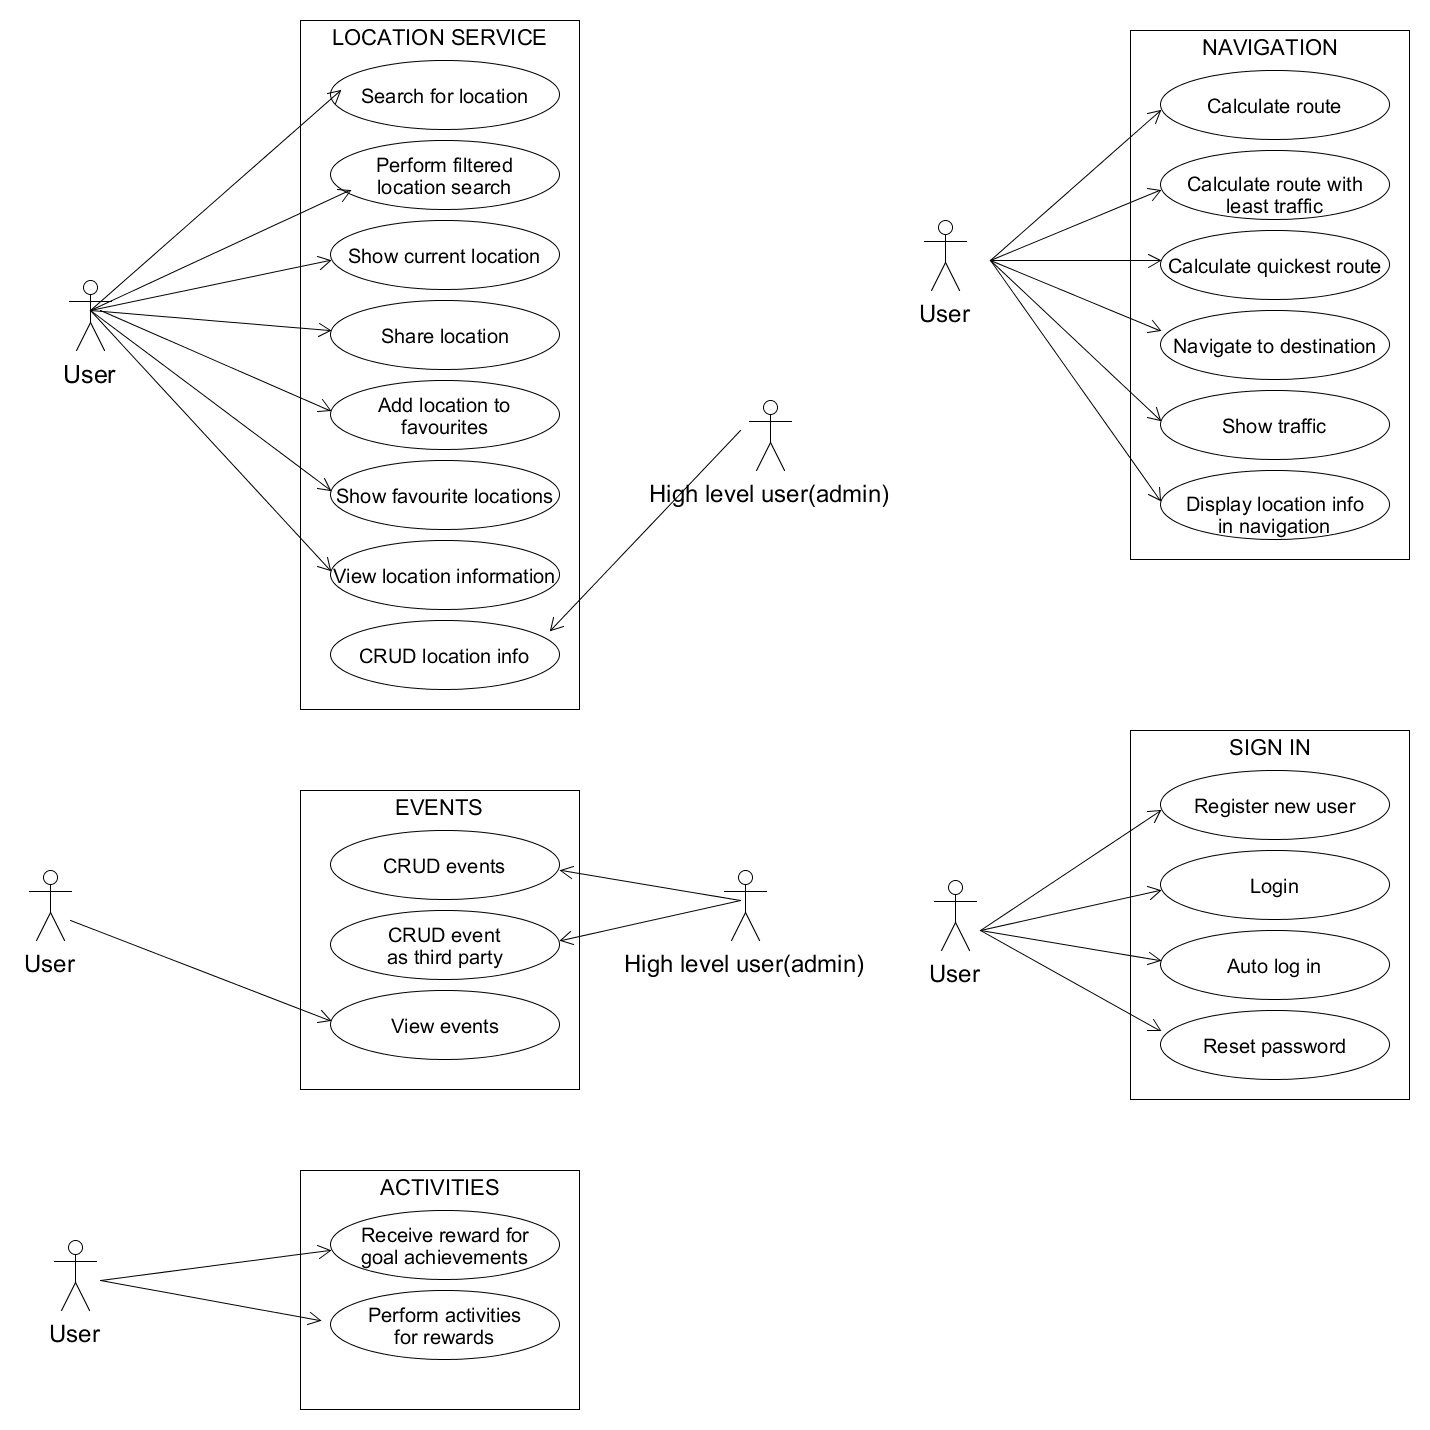
\includegraphics[width=\paperwidth, height=\paperheight]{Images/useCaseDiagrams.png}
	    }\\[2cm]
	    \caption{Use case diagram}
	\end{figure} 
	
	\subsubsection{Actor system interaction}
	\begin{table}[]
		\centering
		\resizebox{\textwidth}{!}{%
			\begin{tabular}{|l|l|}
				\hline
				UC11:Login                          &                           \\ \hline
				Actor: User & System: App           & System : Login Service            \\ \hline
				                                    & App displays home page    \\ \hline
				If user clicks login link           & App displays login page.  \\ \hline
				If user clicks continue link without logging in     & TUCCW navigation. \\ \hline
				TUCEW user sees welcome page        &                            \\ \hline
			\end{tabular}%
		}
	\end{table}
	
	\begin{table}[]
		\centering
		\resizebox{\textwidth}{!}{%
			\begin{tabular}{|l|l|}
				\hline
				UC1:Search for locations    &                                     \\ \hline
				Actor: User                 & System: Location service            \\ \hline
				                            & Location service displays map with the following options \\ \hline
    			TUCBW user either signs in or 
    			continues without signing in   & App displays map with the following options    \\ \hline
				                               & Search for location. \\ \hline
				                               & Perform filtered search for location \\ \hline
				                               & Show current location \\ \hline
				                               & Share location \\ \hline
				                               & Add location to favourites \\ \hline
				                               & Show favourite locations \\ \hline
				                               & View location details \\ \hline
				                               
				TUCEW one of the following cases
                Search for location.                                & \\ \hline
                Perform filtered search for location                & \\ \hline
                Show current location                               & \\ \hline
                Share location                                      & \\ \hline
                Add location to favourites                          & \\ \hline
                Show favourite locations                            & \\ \hline
                View location details                               & \\ \hline
			\end{tabular}%
		}
	\end{table}
	
	\begin{table}[]
		\centering
		\resizebox{\textwidth}{!}{%
			\begin{tabular}{|l|l|}
				\hline
				UC7:Navigate to destination    &                                     \\ \hline
				Actor: User                 & System: Navigation            \\ \hline
				                            & Navigation displays navigation page with the following options \\ \hline
    			TUCBW User sees navigation page   &                         \\ \hline
				                                  & Calculate route without traffic.    \\ \hline
				                                  & Calculate quickest route \\ \hline
				                               
				TUCEW one of the following cases
                Calculate route without traffic. &    \\ \hline
                Calculate quickest route.        &    \\ \hline
			\end{tabular}%
		}
	\end{table}
	
	\begin{table}[]
		\centering
		\resizebox{\textwidth}{!}{%
			\begin{tabular}{|l|l|}
				\hline
				UC5:Calculate route without traffic    &                          \\ \hline
				Actor: User                 &           System: Navigation        \\ \hline
				                            &       User has selected destination \\ \hline
				TUCBW                       &                                      \\ \hline
				                            & App displays home page              \\ \hline
				If user clicks calculate route without traffic button & App determines and displays route on map with least traffic.            \\ \hline \hline
			\end{tabular}%
		}
	\end{table}
	
	\begin{table}[]
		\centering
		\resizebox{\textwidth}{!}{%
			\begin{tabular}{|l|l|}
				\hline
				UC6:Calculate quickest route    &                                     \\ \hline
				Actor: User                 &       System: Navigation               \\ \hline
                                            &       User has selected destination \\ \hline
				TUCBW User clicks "Calculate route" button after selecting destination & \\ \hline
				                            & App displays home page              \\ \hline
				If user clicks calculate quickest route button & App determines and displays quickest route.            \\ \hline \hline
			\end{tabular}%
		}
	\end{table}
	
	\begin{table}[]
		\centering
		\resizebox{\textwidth}{!}{%
			\begin{tabular}{|l|l|}
				\hline
				UC3:Show current location   &                                      \\ \hline
				Actor: User                 &           System: Location service   \\ \hline
				                            &           Map has finished loading \\ \hline
				TUCBW user clicks "show current location" button & Location service determines user location\\ \hline
				                            &           User location and data shown on map     \\ \hline
				\\ \hline
			\end{tabular}%
		}
	\end{table}
	
	\begin{table}[]
		\centering
		\resizebox{\textwidth}{!}{%
			\begin{tabular}{|l|l|}
				\hline
				UC4:Share location    &                                     \\ \hline
				Actor: User                 & System: Location service  \\ \hline
                            				& User is at/selects point of interest \\ \hline
				TUCBW                       &                                      \\ \hline
				If user clicks share button & App shares current location with other app users. \\ \hline \hline
			\end{tabular}%
		}
	\end{table}
	
	\begin{table}[]
		\centering
		\resizebox{\textwidth}{!}{%
			\begin{tabular}{|l|l|}
				\hline
				UC2:Perform filtered search for location    &                     \\ \hline
				Actor: User                 & System: Location service            \\ \hline
				TUCBW search bar is clicked & Filter options are displayed        \\ \hline

				If user clicks on filter button   & App performs search based on filters chosen by user. \\ \hline
				TUCEW user sees search results & \\ \hline
			\end{tabular}%
		}
	\end{table}
	
	\begin{table}[]
		\centering
		\resizebox{\textwidth}{!}{%
			\begin{tabular}{|l|l|}
				\hline
				UC8:Save location to favourites    &                                     \\ \hline
				Actor: User                 &           System: Location service               \\ \hline
				                            & User is at/selects point of interest \\ \hline
				TUCBW "Save location button is pressed" &                          \\ \hline
				If user clicks save location button   & App adds location to list  \\ \hline
				TUCEW confirmation dialog appears           &                           \\ \hline
				                                            & updated favourites list displayed \\ \hline
			\end{tabular}%
		}
	\end{table}
	
	\begin{table}[]
		\centering
		\resizebox{\textwidth}{!}{%
			\begin{tabular}{|l|l|}
				\hline
				UC9:Show favourites   			&                                     \\ \hline
				Actor: User                 		&           System: Location Service       \\ \hline
				TUCBW "Show favourites button is clicked" & App fetches list of favourites from server \\ \hline
				TUCEW favourites page displayed          &                              \\ \hline
			\end{tabular}%
		}
	\end{table}
	
	
	

\begin{table}[]
		\centering
		\resizebox{\textwidth}{!}{%
			\begin{tabular}{|l|l|}
				\hline
				UC10:Registration    &                                     \\ \hline
				Actor: User                 &           System: Login               \\ \hline
				TUCBW                       &                                      \\ \hline
				                            & App displays home page              \\ \hline
				If user clicks login link   & App displays login page.            \\ \hline
				If user clicks continue link without logging in & TUCCW navigation. \\ \hline
				TUCEW user sees home page          &                              \\ \hline
				                                   & User directed to home page
			\end{tabular}%
		}
	\end{table}
	
	\begin{table}[]
		\centering
		\resizebox{\textwidth}{!}{%
			\begin{tabular}{|l|l|}
				\hline
				UC1:Reopen app after closing    &                                   \\ \hline
				Actor: User                 &           System: App               \\ \hline
				                            & App currently minimized/in use\\ \hline
				TUCBW App is reopened       & User signed in automatically  \\ \hline
				                            & App displays home page              \\ \hline
				TUCEW user sees home page   &                              \\ \hline
			\end{tabular}%
		}
	\end{table}	\
	
	\begin{table}[]
		\centering
		\resizebox{\textwidth}{!}{%
			\begin{tabular}{|l|l|}
				\hline
				UC1:Navigation when app is closed    &                                     \\ \hline
				Actor: User                	 &           System: Navigation               \\ \hline
				                           	 &           App running in background\\ \hline
				TUCBW app minimized while navigation in process & \\ \hline
				TUCEW app is reopened/arrival at destination                      &                              \\ \hline
			\end{tabular}%
		}
	\end{table}
	
	\begin{table}[]
		\centering
		\resizebox{\textwidth}{!}{%
			\begin{tabular}{|l|l|}
				\hline
				UC14:Password reset    			   &                                     \\ \hline
				Actor: User                		   & System: Login               \\ \hline
				TUCBW User clicks "forgot password" button & App displays password retrieval page   \\ \hline
				                           		   & App displays home page              \\ \hline
				TUCEW user sees welcome page         	   &                           \\ \hline
			\end{tabular}%
		}
	\end{table}

	\begin{table}[]
		\centering
		\resizebox{\textwidth}{!}{%
			\begin{tabular}{|l|l|}
				\hline
				UC15:Show traffic    			&                                     \\ \hline
				Actor: User                 		&           System: Navigation               \\ \hline
				                           		 & Map already loaded \\ \hline
				TUCBW "Show traffic option is selected" & fetch traffc data and display as heat map\\ \hline
				TUCEW user sees traffic data on map      &                              \\ \hline
			\end{tabular}%
		}
	\end{table}
	
	\begin{table}[]
		\centering
		\resizebox{\textwidth}{!}{%
			\begin{tabular}{|l|l|}
				\hline
				UC1:User walks past location he will be interested in    &                                     \\ \hline
				Actor: User                 &           System: App               \\ \hline
				TUCBW                       &                                      \\ \hline
				TUCEW                        &                              \\ \hline
			\end{tabular}%
		}
	\end{table}
	
	\begin{table}[]
		\centering
		\resizebox{\textwidth}{!}{%
			\begin{tabular}{|l|l|}
				\hline
				UC1:Block notifications    &                                     \\ \hline
				Actor: User                 &  System: Notification               \\ \hline
				TUCBW                       &                                      \\ \hline
				TUCEW          &                              \\ \hline
			\end{tabular}%
		}
	\end{table}
	
	\begin{table}[]
		\centering
		\resizebox{\textwidth}{!}{%
			\begin{tabular}{|l|l|}
				\hline
				UC1:View location information    &                                     \\ \hline
				Actor: User                 &           System: App               \\ \hline
				TUCBW                       &                                      \\ \hline
				                            & App displays home page              \\ \hline
				If user clicks login link   & App displays login page.            \\ \hline
				If user clicks continue link without logging in & TUCCW navigation. \\ \hline
				TUCEW user sees welcome page          &                              \\ \hline
			\end{tabular}%
		}
	\end{table}
	
	\begin{table}[]
		\centering
		\resizebox{\textwidth}{!}{%
			\begin{tabular}{|l|l|}
				\hline
				UC1:CRUD location information    &                                     \\ \hline
				Actor: User                 &           System: App               \\ \hline
				TUCBW                       &                                      \\ \hline
				TUCEW  &                              \\ \hline
			\end{tabular}%
		}
	\end{table}
	
	\begin{table}[]
		\centering
		\resizebox{\textwidth}{!}{%
			\begin{tabular}{|l|l|}
				\hline
				UC1:User gets reward    &                                     \\ \hline
				Actor: User                 &           System: Activities               \\ \hline
				TUCBW                       &                                      \\ \hline
				                            & App displays home page              \\ \hline
				If user clicks login link   & App displays login page.            \\ \hline
				If user clicks continue link without logging in & TUCCW navigation. \\ \hline
				TUCEW user sees welcome page          &                              \\ \hline
			\end{tabular}%
		}
	\end{table}
	
	\begin{table}[]
		\centering
		\resizebox{\textwidth}{!}{%
			\begin{tabular}{|l|l|}
				\hline
				UC1:User walks required steps    &                                     \\ \hline
				Actor: User                 &           System: Activities               \\ \hline
				TUCBW                       &                                      \\ \hline
				                            & App displays banner message              \\ \hline
				If user takes no action wait & App displays login page.            \\ \hline
				Click banner or open app to retrieve reward & Rewards page displayed. \\ \hline
				TUCEW banner message disappears after set time & \\ \hline
			\end{tabular}%
		}
	\end{table}
	
	\begin{table}[]
		\centering
		\resizebox{\textwidth}{!}{%
			\begin{tabular}{|l|l|}
				\hline
				UC1:CRUD events    &                                     \\ \hline
				Actor: User                 &           System: App               \\ \hline
				                            & App displays home page              \\ \hline
				                            TUCBW                       &                                      \\ \hline
				If user clicks login link   & App displays login page.            \\ \hline
				If user clicks continue link without logging in & TUCCW navigation. \\ \hline
				TUCEW user sees welcome page          &                              \\ \hline
			\end{tabular}%
		}
	\end{table}
	
	\begin{table}[]
		\centering
		\resizebox{\textwidth}{!}{%
			\begin{tabular}{|l|l|}
				\hline
				UC23:Create event as third party   	&                                     \\ \hline
				Actor: User                 		&           System: Events               \\ \hline
				TUCBW "Create event" button is clicked  & Page displayed to capture details  \\ \hline
				If user clicks continue link without logging in & TUCCW navigation. \\ \hline
				TUCEW user sees welcome page         	 &                              \\ \hline
			\end{tabular}%
		}
	\end{table}
	
	\subsubsection{Traceability Matrix}
	\begin{table}[ht!]
		\centering
		\label{Trac}
		\resizebox{\textwidth}{!}{%
			\begin{tabular}{|c|c|c|c|c|c|c|c|c|c|c|c|c|c|c|c|c|c|c|c|c|c|c|c|c|}
				\hline
				Requirement & Priority & UC1 & UC2 & UC3 & UC4 & UC5 & UC6 & UC7 & UC8 & UC9 & UC10 & UC11 & UC12 & UC13 & UC14 & UC15 & UC16 & UC17 & UC18 & UC19 & UC20 & UC21 & UC22 & UC23 \\ \hline
				FR1 & 3 &  &  &  &  &  &  &  &  &  & X &  &  &  &  &  &  &  &  &  &  &  &  &  \\ \hline
				FR2 & 3 &  &  &  &  &  &  &  &  &  &  & X & X &  &  &  &  &  &  &  &  &  & X & X \\ \hline
				FR3 & 3 &  &  &  &  &  &  &  & X & X & X & X &  &  & X &  &  &  &  &  &  &  &  &  \\ \hline
				FR4 & 3 &  &  &  &  &  &  &  &  &  &  &  &  &  & X &  &  &  &  &  &  &  &  &  \\ \hline
				FR5 & 5 & X & X &  &  &  &  &  &  &  &  &  &  &  &  &  &  &  &  &  &  &  &  &  \\ \hline
				FR6 & 6 &  &  & X & X &  &  &  & X &  &  &  &  &  &  &  & X &  & X &  &  &  &  &  \\ \hline
				FR7 & 6 &  &  &  &  & X & X & X &  &  &  &  & X & X &  &  &  &  &  &  &  &  &  &  \\ \hline
				FR8 & 4 &  &  &  &  & X &  &  &  &  &  &  &  &  &  & X &  &  &  &  &  &  &  &  \\ \hline
				FR9 & 5 &  &  &  &  &  &  &  &  & X &  &  &  &  &  &  &  &  &  & X & X &  &  &  \\ \hline
				FR10 & 4 &  &  &  &  &  &  &  &  &  &  &  &  &  &  &  & X & X &  &  &  &  &  &  \\ \hline
				FR11 & 3 &  &  &  &  &  &  &  &  &  &  &  &  &  &  &  &  &  &  &  & X &  &  &  \\ \hline
				FR12 & 1 &  &  &  &  &  &  &  &  &  &  &  &  &  &  &  &  &  &  &  &  & X &  &  \\ \hline
				FR13 & 3 &  &  &  &  &  &  &  &  &  &  &  &  &  &  &  &  &  &  &  &  &  & X & X \\ \hline
				\multicolumn{2}{|c|}{UC Priority} & 5 & 5 & 6 & 3 & 5 & 5 & 5 & 6 & 3 & 3 & 4 & 3 & 3 & 4 & 5 & 4 & 2 & 6 & 6 & 3 & 2 & 4 & 4 \\ \hline
			\end{tabular}%
		}
	\end{table}
	

\end{document}
